\section{The GCard Framework}
\label{sec:overview}

%% TODO


%%% BY CODEX !!!!

\begin{figure*}[!b]
  \centering
  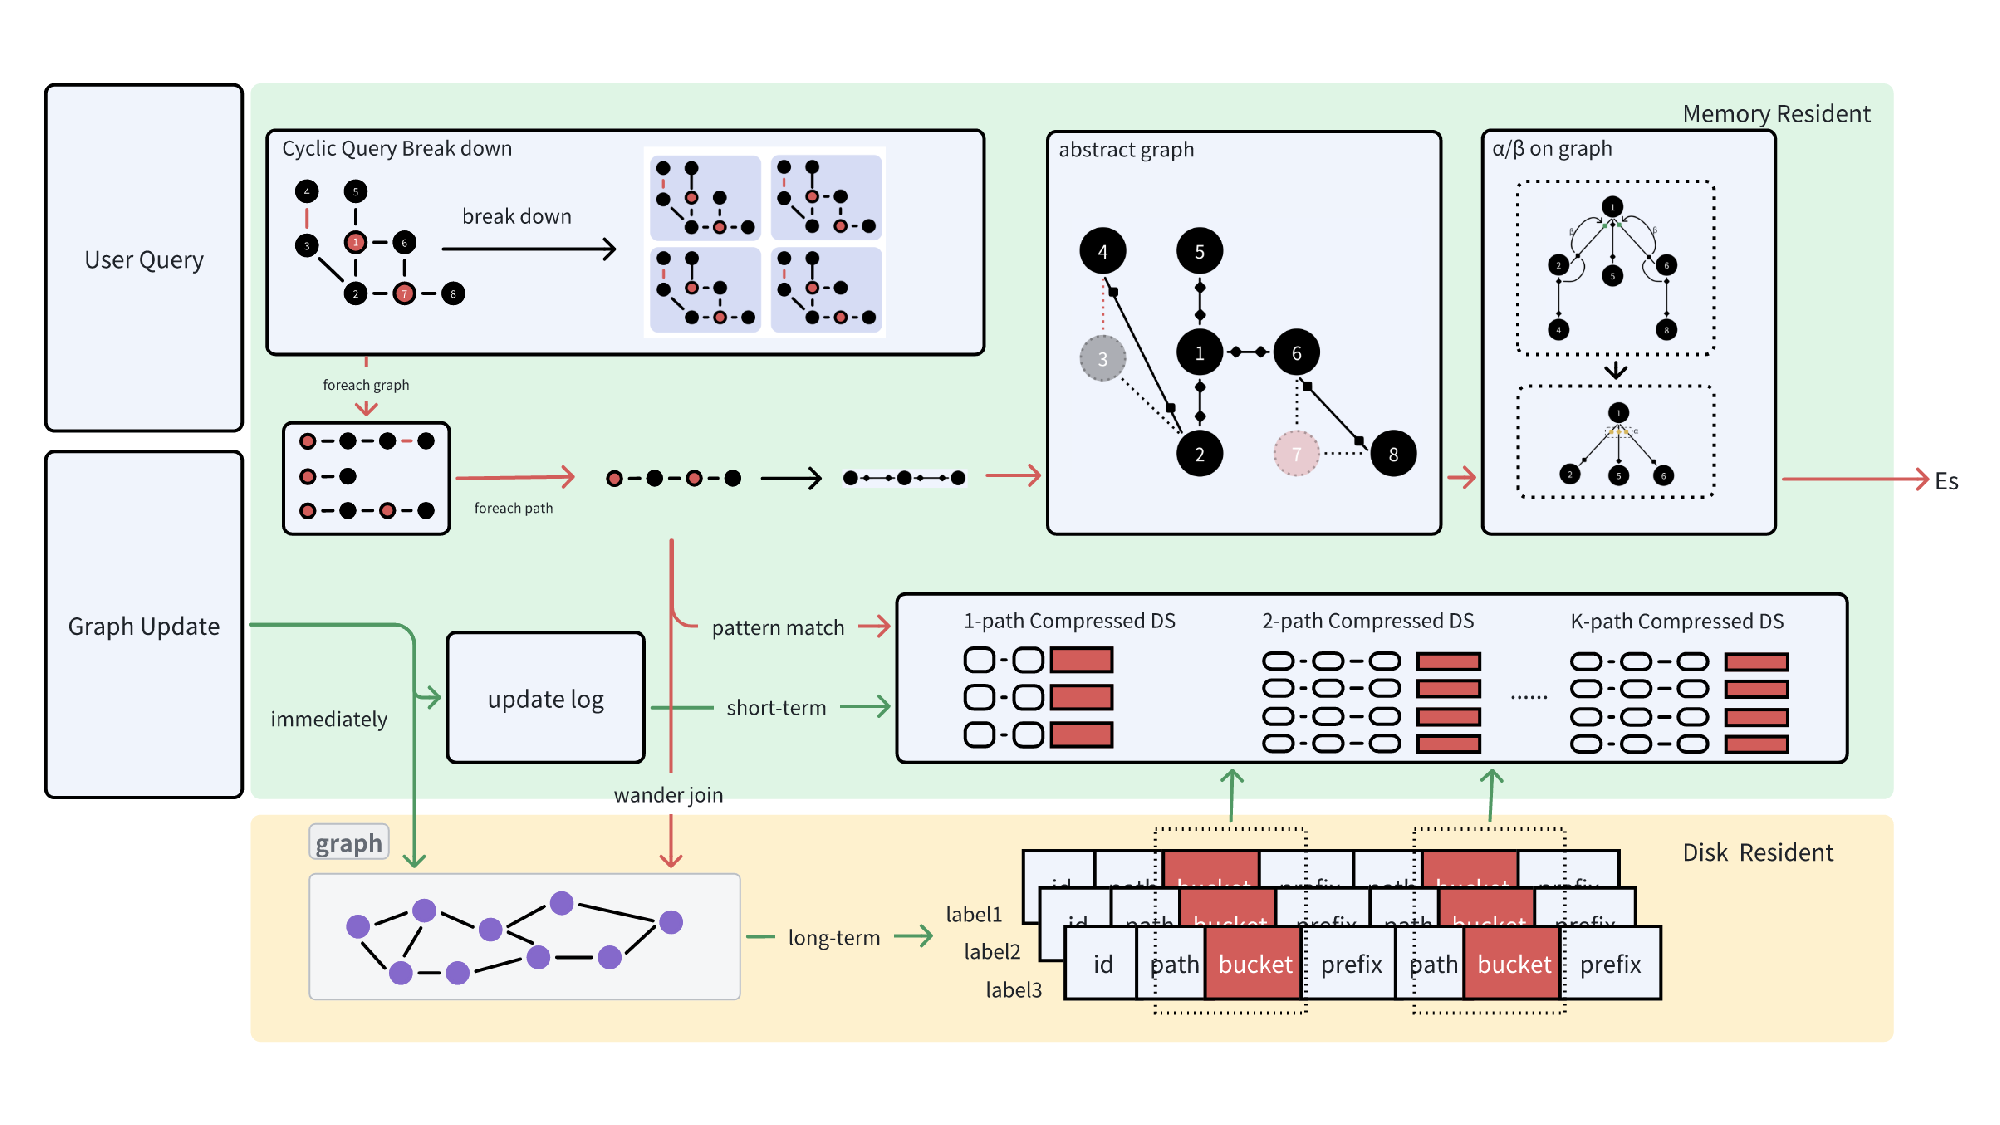
\includegraphics[width=\textwidth]{figures/sec-framework/framework_v1.pdf}
  \caption{Overview of GCard.}
  \label{fig:overview}
\end{figure*}

\stitle{PathDS: An Update-Friendly Summary}. \eat{At the core of GCard is
PathDS, a compact summary of path-level degree statistics. For each
degree value $d$, PathDS stores only a short high-order bit prefix
(e.g., 4 or 8 bits) and the highest-bit position, rather than the full
64-bit integer. During inference, GCard reconstructs a conservative value
$\hat d$ from this code such that $\hat d \ge d$, preserving an upper-bound
view of degree statistics. Because each update only changes the local
codes of affected paths, PathSketch supports efficient incremental
maintenance without rebuilding all summaries.}


\stitle{A Predicate Decoupling Design}. \eat{A key design principle of GCard
is predicate decoupling. Instead of materializing many
predicate-conditioned summaries offline, GCard keeps one structural
PathSketch and estimates predicate effects online as path-attached
selectivity factors. This design separates structural maintenance from
predicate handling, so data updates trigger only structural summary
updates, while predicate selectivity is evaluated at query time using a
conservative correction strategy.}

\stitle{A Cycle-Aware Estimation Algorithm}. \eat{For cyclic queries, GCard
first rewrites the query into an acyclic surrogate by removing a small
set of cycle-closing edges selected by a lightweight rule. It then
estimates the acyclic core with PathSketch and applies a conservative
recovery factor for the removed edges. This cycle-to-acyclic pipeline
keeps inference tractable while retaining conservative estimates on
cyclic workloads.}
